\subsection{Subjects and electrode placement}

The experiment was carried out on ten healthy subjects, two women and
eight men, nine right-handed and one left-handed, of an average age of
$30.9 \pm 8.45$ years. The subjects were given no knowledge of what
the experiment was about. We placed on each subject's dominant forearm
$7$ surface EMG electrodes, according to this anatomic guideline:

\begin{itemize}

  \item on the forearm ventral side: near the wrist, above the
    \emph{flexor pollicis longus}; centrally, above the \emph{flexor
    digitorum superficialis}; near the elbow, above the \emph{flexor
    digitorum profundus}; and near the wrist, above the \emph{flexor
    digitorum superficialis} again;

  \item on the forearm dorsal side: near the wrist, above the
    \emph{extensor pollicis brevis / abductor pollicis longus};
    centrally, above the \emph{extensor digitorum communis} and
    \emph{extensor digiti minimi}.

\end{itemize}

These positions were chosen, according to the medical literature
\cite{Kendall},
as carefully as possible in order to identify the best EMG sources and
to detect the activity of the most relevant flexor and extensor
muscles of the forearm. It must be noted, however, that we detected,
both visually and by palpation, that inter-arm differences are
remarkable, depending on the subjects' age, gender and physical
fitness. Moreover, some of the aforementioned muscles are deep into
the forearm, so that muscle cross-talk cannot be avoided. This is a
well-known problem in the EMG literature (\cite{deluca,zecca}) and is
one of the factors that make our problem hard: it is like
reconstructing a coherent speech by listening to $19$ people who talk
at the same time, and not necessarily the ones we want to listen to
are the loudest and clearest speakers in the room.

\subsection{Sensors and hardware}

\begin{figure*}[!t] \centering
  \begin{tabular}{ccc}
    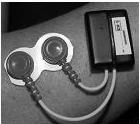
\includegraphics[height=0.16\textheight]{figs/Electrode} &
    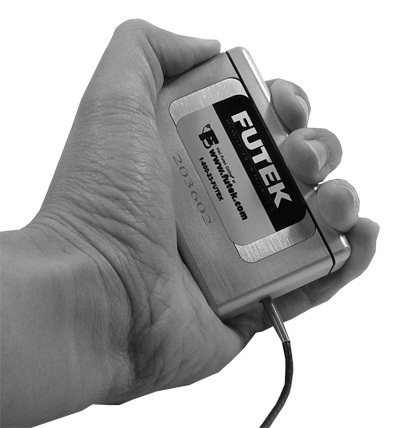
\includegraphics[height=0.16\textheight]{figs/Hand_Gripper} &
    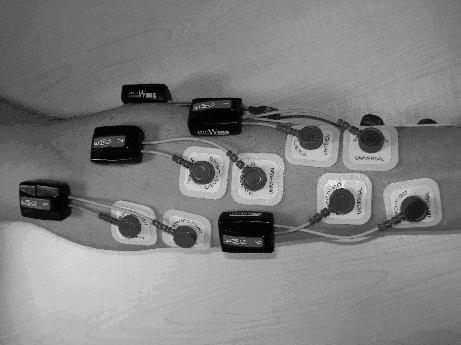
\includegraphics[height=0.16\textheight]{figs/El_Arrangement} \\
    $(a)$ & $(b)$ & $(c)$ \\
  \end{tabular}
  \caption{The experimental setup (\textit{subject side}): $(a)$ an EMG
    wireless electrode; $(b)$ the FUTEK force sensor; $(c)$ the typical
    placement of the EMG electrodes on a subject's forearm (ventral side).}
  \label{fig:SubjSetup}
\end{figure*}

The electrodes we employed are Aurion ZeroWire wireless surface EMG
electrodes (see \cite{zerowire}). The use of wireless electrodes is
particularly appreciated in such kind of experiments, since the
subjects would eventually have to be free to perform DLA-like actions
during the experiment, i.e., in a specific phase of the experiment
they were allowed to walk around, pronate and supinate their forearms,
sit down and stand up, walk, etc. Wireless electrodes let the subjects
feel free.

Each subject was also given a FUTEK LMD500 Hand Gripper force sensor
(see \cite{LMD500}) in order to detect the force applied by the subjects'
hand during the experiment.

Figure \ref{fig:SubjSetup} shows $(a)$ a single electrode, glued to
the subject's forearm skin; $(b)$ the force sensor as gripped during a
power grasp; and $(c)$ the typical placement of the electrodes
(ventral side of the forearm).

It is well-known that the EMG raw signal relevant bandwidth lies
between $15$ and $500$Hz, so we set the sampling rate at $2$KHz. In
order to avoid synchronisation problems, the same sampling rate was
applied to the force sensor, although we obviously expect a much lower
bandwidth from this sensor than from the EMG sensors.

We used a standard National Instruments data acquisition board
(NI-USB6211) to record the sensors' signals, connected to the receiver
of the EMG wireless device (Figure \ref{fig:ExpSetup}) and to an
amplifier connected to the force sensor. The board was connected via a
USB port to an entry-level laptop. We used a custom National
Instruments' LabView VI block to acquire the signals.

\begin{figure*}[!t] \centering
  \begin{tabular}{cc}
   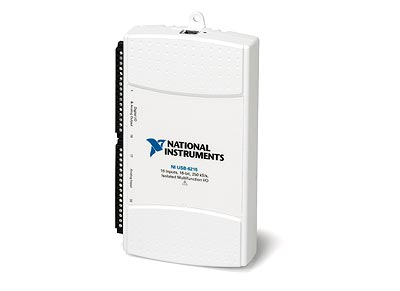
\includegraphics[height=0.16\textheight]{figs/NI-6211} &
    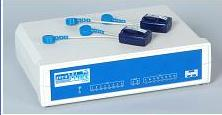
\includegraphics[height=0.16\textheight]{figs/Zero_Base} \\
  $(a)$ & $(b)$\\
  \end{tabular}
  \caption{The experimental setup (\textit{experimenter side}): $(a)$
   the USB data acquisition card (NI-USB6211); $(b)$ the EMG device
   receiver.}
  \label{fig:ExpSetup}
\end{figure*}

\subsection{Experiment design}

The experiment consisted of two phases, one right after the
other.

During phase $1$ the subject would keep her/his arm still and relaxed
on a table, and was asked to grasp the force sensor using, in turn,
three different grips (Figure~\ref{fig:Grasps}):

\begin{itemize}
  \item index precision grip;
  \item other fingers precision grip;
  \item power grasp.
\end{itemize}

\begin{figure*}[!t] \centering
  \begin{tabular}{ccc}
   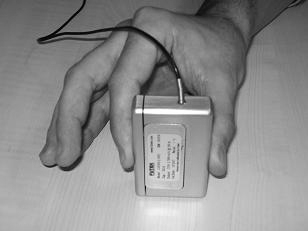
\includegraphics[height=0.16\textheight]{figs/grip1} &
    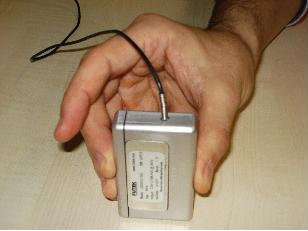
\includegraphics[height=0.16\textheight]{figs/grip2} &
    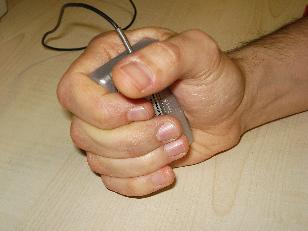
\includegraphics[height=0.16\textheight]{figs/grip3} \\
    $(a)$ & $(b)$ & $(c)$ \\
  \end{tabular}
  \caption{The three different grips employed in the experiment: $(a)$
   index precision grip; $(b)$ other fingers precision grip; $(c)$
   power grasp.}
  \label{fig:Grasps}
\end{figure*}

A rest condition was sampled beforehand to define the baseline of the
EMG activity. The subject freely repeated each grasping action for
$100$'', resting for $30$'' in between grasps. The whole procedure was
repeated twice, in order to gather more data and diminish the effect
of local, statistically irrelevant, errors. Since during these
activities the subject would lie in a highly controlled position
(relaxed arm and sitting posture), this phase will
be referred to from now on as the \emph{Still-Arm phase (SA)}.

Phase $2$, actually the more interesting one for the final intent of
this study, consisted in repeating phase $1$ in a less controlled
condition: the subject was asked to grasp the force sensor while
freely moving, walking around, lifting and pronating / supinating the
arm and forearm, sitting down and standing up from a chair; this would
emulate the main movements that one is expected to do during his DLAs.
This second phase will be called \emph{Free-Arm phase (FA)}.

As a whole, each subject's experiment resulted in something more than
$1200$'' of data; at the above mentioned sampling rate of $2$KHz, this
makes it for about $2.4\times 10^6$ samples for each subject, equally
distributed in each phase.

\subsection{Data pre-processing}

Unlike commercial EMG electrodes, such as, e.g., Otto Bock's MyoBock
electrodes \cite{ottobock}, the electrodes employed here would return
the ``raw'' EMG signal, without any low-pass filtering or Root-Mean
Square (RMS) processing. Nevertheless, it is well-known (see, again,
\cite{deluca,zecca}) that muscular activity, namely the force exerted
by a muscle, is strongly related to the RMS of the EMG signal, rather
than to the raw signal. For this reason, and also in order to aim at a
more practical, commercial implementation, we decided to evaluate the
RMS of the obtained EMG signals, electrode by electrode.

For a given mono-variate discrete time-varying signal, the RMS is
defined as the mean of the squares of the signal values, evaluated
over a certain time-window $T_{RMS}$. Roughly speaking, the RMS acts
like an envelope extraction plus a low-pass filter, whose cutoff
frequency grows smaller as the time-window grows larger (i.e., as
$T_{RMS}$ becomes higher). For this reason, high values of $T_{RMS}$
imply an ostensible delay in the resulting signal that is due to
\emph{responsiveness} of the synthesized output signal. It becomes
slower and slower as the $T_{RMS}$ value increases, since more samples
must be stored before a significant value can be evaluated.  The
choice of $T_{RMS}$ is therefore crucial in order to produce a signal
which is maximally related to the force signal, unaffected by
high-frequency noise, and with an acceptable lag. However, it must be
noted here that the EMG signal, being directly related to the muscle
\emph{activation potentials}, happens to \emph{anticipate} the muscle
movements by a few hundreds milliseconds\footnote{The
electromechanical delay (EMD) of a muscle is defined as the interval
between the onset of the electrical activity of the muscle (EMG)
indicating its activation by the neural system and the onset of the
resulting change in the mechanical variable observed. The delays
reported range from 25 to 100 ms for different muscles and tasks
\cite{Wolf1994}.}; therefore, in a practical application, a wider lag
is acceptable than one would expect. This is useful since it allows us
to increase $T_{RMS}$, if necessary.

\begin{figure*}[!ht] \centering
  \begin{tabular}{cc}
    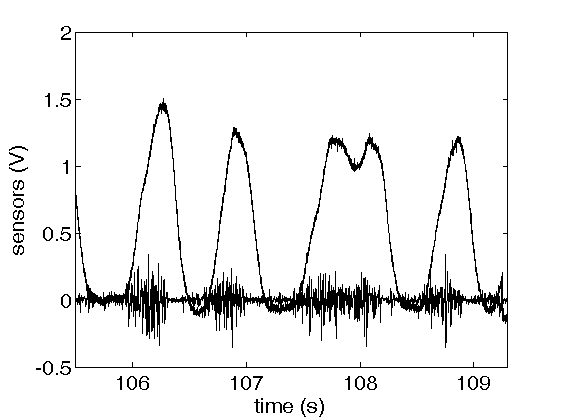
\includegraphics[width=0.45\textwidth]{figs/force_raw} &
    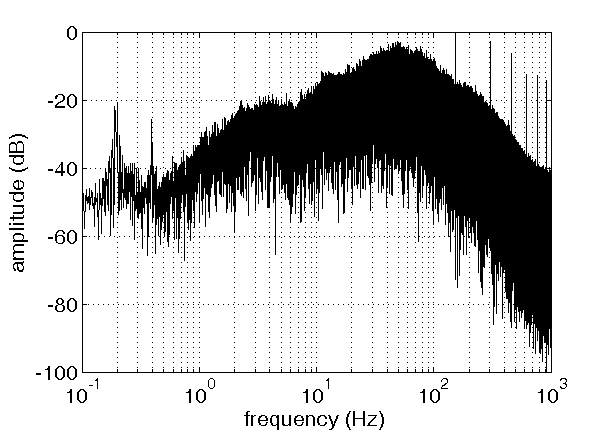
\includegraphics[width=0.45\textwidth]{figs/spectrum_raw} \\
    $(a)$ & $(b)$ \\
  \end{tabular}
  \caption{$(a)$ typical raw EMG and force signals (the EMG signal
    being the bottom, high-frequency one); $(b)$ frequency diagram of
    the EMG signal.}
  \label{fig:spectra}
\end{figure*}

\begin{figure*}[!ht] \centering
  \begin{tabular}{ccc}
    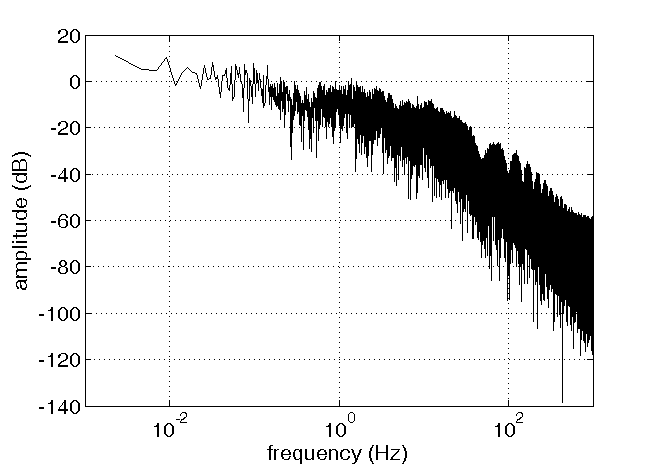
\includegraphics[width=0.3\textwidth]{figs/spectrum_RMS0040} &
    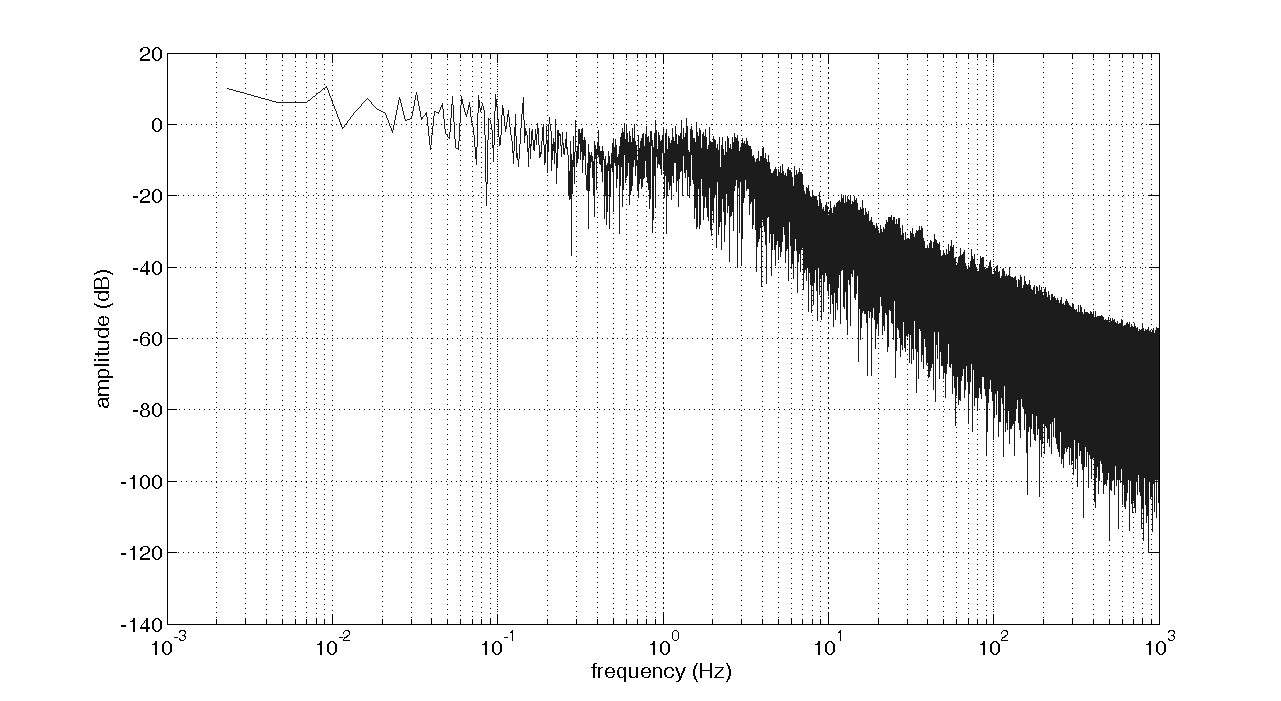
\includegraphics[width=0.3\textwidth]{figs/spectrum_RMS0200} &
    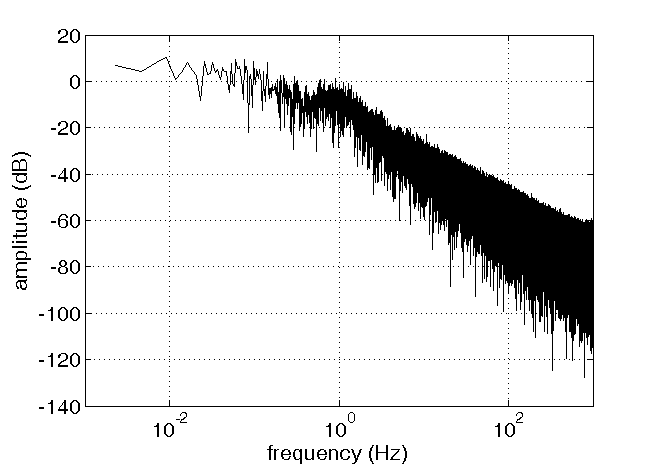
\includegraphics[width=0.3\textwidth]{figs/spectrum_RMS1000} \\
    $(a)$ & $(b)$ & $(c)$ \\
  \end{tabular}
  \caption{(left to right) effects of the RMS on the bandwidth of the EMG
    signals, for $T_{RMS} = 20, 100, 500ms$.}
  \label{fig:RMSs}
\end{figure*}

Unfortunately we are unaware of any systematic way of setting a good
value of $T_{RMS}$ in such a framework; the Otto Bock electrodes' one
is not mentioned either in the related technical specification
sheet. Therefore we found $T_{RMS}$ heuristically, according to some
initial experiments. See the next Section for more details. As an
example, though, consider Figures \ref{fig:spectra} and
\ref{fig:RMSs}.

Figure \ref{fig:spectra} (panel $(a)$) shows a few seconds of typical
force / EMG behaviour: it is apparent that the EMG signal (the bottom
one, with high frequencies) starts oscillating when the force signal
(the top one) starts increasing. It is also quite clear that the
amplitude of the envelope of the EMG is related to the force, as is
indicated in literature. Panel $(b)$ shows the frequency analysis of
the same EMG signal: as one can see, the meaningful bandwidth lies in
the interval known from the literature.

On the other hand, Figure \ref{fig:RMSs} shows the effect of the RMS
on the frequency components of the EMG, for three different values of
$T_{RMS}$. It is clear that the meaningful bandwidth now contains all
low-frequency components, possibly down to the constant, and is
upper-bounded by about $25$Hz (panel $(a)$, for $T_{RMS}=20ms$) to
$10$Hz (panel $(c)$, for $T_{RMS}=0.5s$). As expected, larger values
of $T_{RMS}$ correspond to a better filtering but also to a larger
delay.

This enables us to safely sub-sample the EMG signal after the RMS has
been applied. Assuming that $T_{RMS}$ is not too small, we have
subsampled both the EMG and force signal at $25$Hz, taking one sample
in $80$ of the original sequence. This has considerably reduced the
amount of data to be processed, namely to about $30.000$ samples for
each subject.

As a last data pre-processing step, we removed from the sample set
those samples for which the applied force was lower than a specific
threshold, in order to get a clearer representation of the activation
potentials. This threshold was chosen in order to remove a minimal
fraction of the samples. Of course, we fully retained the samples
corresponding to the baseline rest condition. This is why we preferred
to record this condition before the rest of the experiment.

\subsection{Support Vector Machines}

According to \cite{2008.ICRA,2008.BioCyb}, where a detailed
comparative analysis among three different machine learning methods
was carried out, we chose to employ Support Vector Machines (SVMs) to
solve our problem. For an explanation of how SVMs work in the context
of EMG signals, please refer to those papers; for a comprehensive
tutorial on SVMs in the more general framework of
\emph{classification} and \emph{regression}, refer to
\cite{Burges98,SmolaTut2004}.

Suffice it here to say that SVMs are a statistical learning method
able to build an approximated map between an input space and a label
(classification) or a real value (regression). Classification is here
used to classify the type of grasp according to the EMG signal,
whereas regression is used to understand how much force the subject is
exerting, independently from the grasp type; the input space is then
$\RR^7$, one coordinate for each EMG electrode; the labels are four
integer numbers, one for each grasp type; and the real value is
exactly the force value read off the force sensor.

SVMs are a \emph{supervised learning} approach, meaning that they must
first be \emph{trained} on an EMG dataset for which labels and force
values are known, in order to build the required input/output map; and
then they can be used to \emph{predict} the values of new EMG samples,
using the map. Notice that we work in real-time, that is, our machines
associate a grasp type and a force value to an EMG value \emph{at each
instant of time}. This approach enables us to detect a grasp type
\emph{almost at the onset of the grasping movement}\footnote{the
precise onset of the movement would correspond to those samples which
were removed since they were associated to too low a force value.},
differently from what happens in other approaches (e.g.,
\cite{smagt,Sebelius2005}) in which all values of the input signal over a
further time-window are employed as the input space, in order to let
the system understand better the final grasp type.

Lastly, SVMs are known to suffer from heavy computational needs when
it comes to training on large datasets: training on these datasets
would have then been prohibitive. Moreover, the general aim of our
research is to build an on-line system, able to predict in a very
short amount of time; and in on-line learning the flow of training
data is potentially endless. So we need a way of checking whether the
EMG samples used for training are useful, rejecting the ones deemed
useless. This is supposed to eventually keep the training set bounded,
and dramatically reduce the training set size in this particular
experiment, where the training time is rather small if compared to a
real-life setting. We employ \emph{uniformisation}
\cite{2008.ICRA,2008.BioCyb} to do this: given a \emph{minimum
distance} $d > 0$, we reject those samples which are too close to each
other, with the underlying assumption that the maps we are trying to
build are smooth enough to allow such a simplification. More in
detail, the samples in a training batch are considered one by one in
chronological order, as it would happen in an on-line setting; each
new sample is then added to the training set if, and only if, its
distance from all training samples retained so far is at least
$d$.

\begin{figure*}[!ht] \centering
  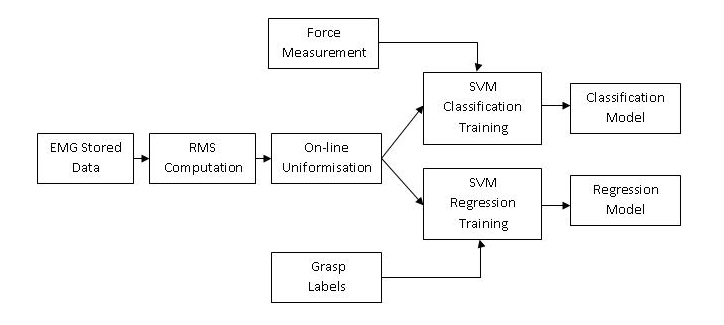
\includegraphics[width=0.75\textwidth]{figs/Schema} \\
  \caption{Graphical representation of the system employed to solve our problem.}
  \label{fig:Algorithm}
\end{figure*}

Figure \ref{fig:Algorithm} graphically depicts the structure of our
system, finally producing the classification and regression models,
which will be then used for the prediction. Notice that there can
actually be two different RMS windows, one for classification and one
for regression.
